\chapter{Future Work \& Planning}
\label{cha:planning}
\section{Intro}
\label{sec:planningIntro}
The initial stage of this project 
was simultaneously done with other UCs 
(CDLE, ASI, ES, CD) and focused on 
studying and understanding the problem,
while analyzing existing \gls{eRange} solutions.
From then, researching usable a \gls{dataset}
was prioritized as it would prove vital
for testing the study's model.
After choosing two equally valid \glspl{dataset}
\citep{vedDataset, emobpy}, the new focus for 
this study shifted into implementing an existing
solution of the "basic", and adaptive history 
based model approaches proposed by \citep{classicEVX}.
While also writing this report,
additional research on existing related works 
was conducted for better understanding
of the problem regarding \gls{eRange} estimation, 
its difficulties and the existing 
\gls{machineLearning} solutions.

\vbox{

\section{Planning}
\label{sec:planningPlanning}

The figure bellow details the planning of 
the following months of work for this project. 

\begin{figure}[H]
    \begin{center}
        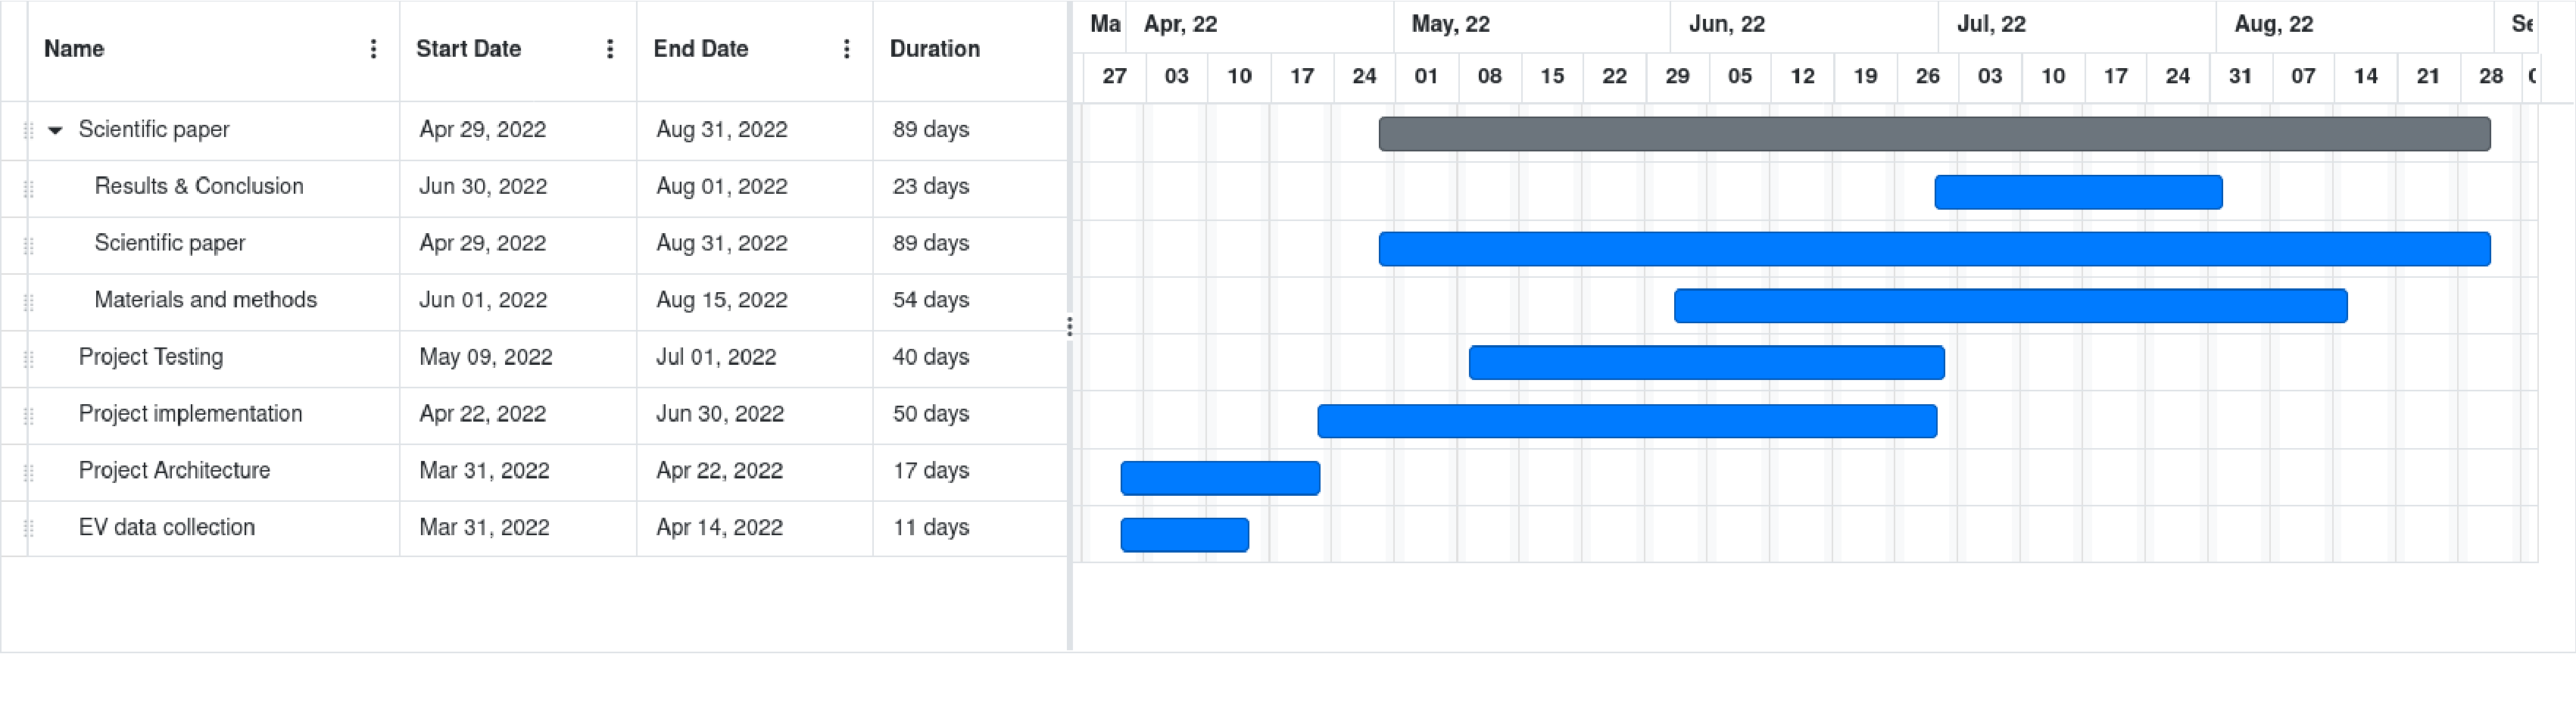
\includegraphics[scale=0.20]{../figures/planning}
        \caption{Project planning.}
    \end{center}
\end{figure}

The project development will be separated into three 
separate stages: Project Architecture, 
Project Implementation, and Project Testing.
Project Architecture stage will plan the software
architecture to develop, this stage will continue 
after Project Implementation has started, allowing
future adjustments according to implementation demands.
The required software to have a working model on this project
will be developed during the Implementation stage,
having the following milestones: \Gls{dataset} integration, 
and Implemented Model. The Project Testing stage
will ascertain the validity of the estimated results. 
During the previously mentioned project stages, 
thesis writing will be continually worked until
its completion, depending on Project Testing stage
to reflect on the projects results and accomplishments.

}

